
\section{Wrap Spring Knee Orthosis}
\label{sec:knee}

The work done in this section was in collaboration with  Vishnu Aishwaryan \cite{mani2020design}. I managed the overall mechanical design and the manufacturing process. I also aided in the design and running of the experimental validation.

Despite the body of literature about knee orthosis, only a few report the essential quantitative measurements, such as static or dynamic torque, safety, weight, and size. The lack of critical information made it difficult to arrive at design criteria. The design of the knee orthosis was based on the design criteria, and the trade study found here \cite{subra2020design}. In the trade study, each criterion was assigned a different weight of importance, totaling 100 points, and allowed for the mechanism and parameters for the knee orthosis to be selected. The study concluded that a wrap spring clutch mechanism was the best design due to its highest score. The results are summarized in \autoref{tab:trade}.


\begin{table}[h!]
  \begin{center}
    \begin{tabular}{c|c|c|c} % <-- Alignments: 1st column left, 2nd middle and 3rd right, with vertical lines in between
      \textbf{wrap spring} & \textbf{motor} & \textbf{gears/clutch} & \textbf{cables} \\
      \hline \hline
      832.5 & 627.5 & 752.5 & 675.0 \\
      \hline
      \textbf{SEA}  & \textbf{Wafer disks}  & \textbf{Mag Damper} & \textbf{Hydraulics} \\
      \hline \hline
      592.5 & 805.0 & 757.5 & 580.0\\
    \end{tabular}
  \end{center}
      \caption[Knee Trade Study]{Summery of trade study}
    \label{tab:trade}
\end{table}


A wrap spring clutch mechanism is a quasi passive mechanism that allows for high holding torques \cite{irby1999optimization} \cite{tung2013design}. It consists of an arbor that is concentric with a wrap spring. \autoref{fig:WrapSpringClutch} illustrates how a wrap spring clutch mechanism works. The arbor is designed to have a slightly larger diameter than the spring. The friction between the arbor and spring prevents the arbor from rotating. When the leg's spring is actuated, the spring's diameter increases, allowing the spring to rotate freely. 

\begin{figure}
    \centering
    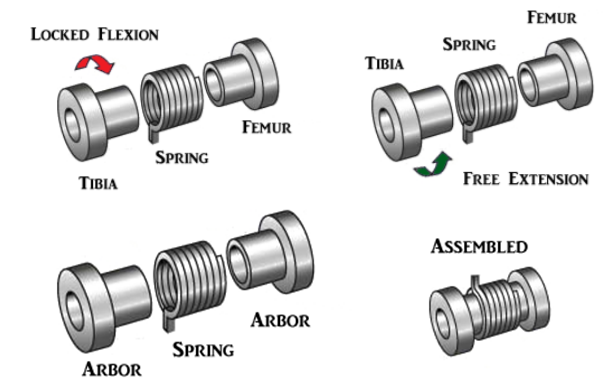
\includegraphics[scale=0.45]{images/mech_design/wrapspringclutch.png}
    \caption[Wrap Spring Clutch]{Diagram of how a wrap spring clutch functions. The spring prevent rotation in one direction while locked and free motion when the spring is opened. \cite{irby1999optimization}}
    \label{fig:WrapSpringClutch}
\end{figure}


The knee joint for LARRE uses a wrap spring clutch/brake mechanism. \autoref{fig:kneemechASM} shows the knee casing and components.  \autoref{fig:subknee} shows the primary knee mechanism and all the components that comprise the sub-assemblies. The brake engages to lock the knee joint during the stance phase to prevent possible knee flexion and release during the swing phase. The knee's joint consists of a central shaft over which the arbor was mounted via a set screw. The spring wraps around this setup to produce the clutching/braking effect. One end of the spring clamped between the end cover and thigh link, which held the spring in place. A potentiometer is connected to the center shaft to measure joint angles during walking gait.


\begin{figure}
    \begin{subfigure}{\textwidth}
        \centering
        \captionsetup{justification=centering}
        \centerline{
        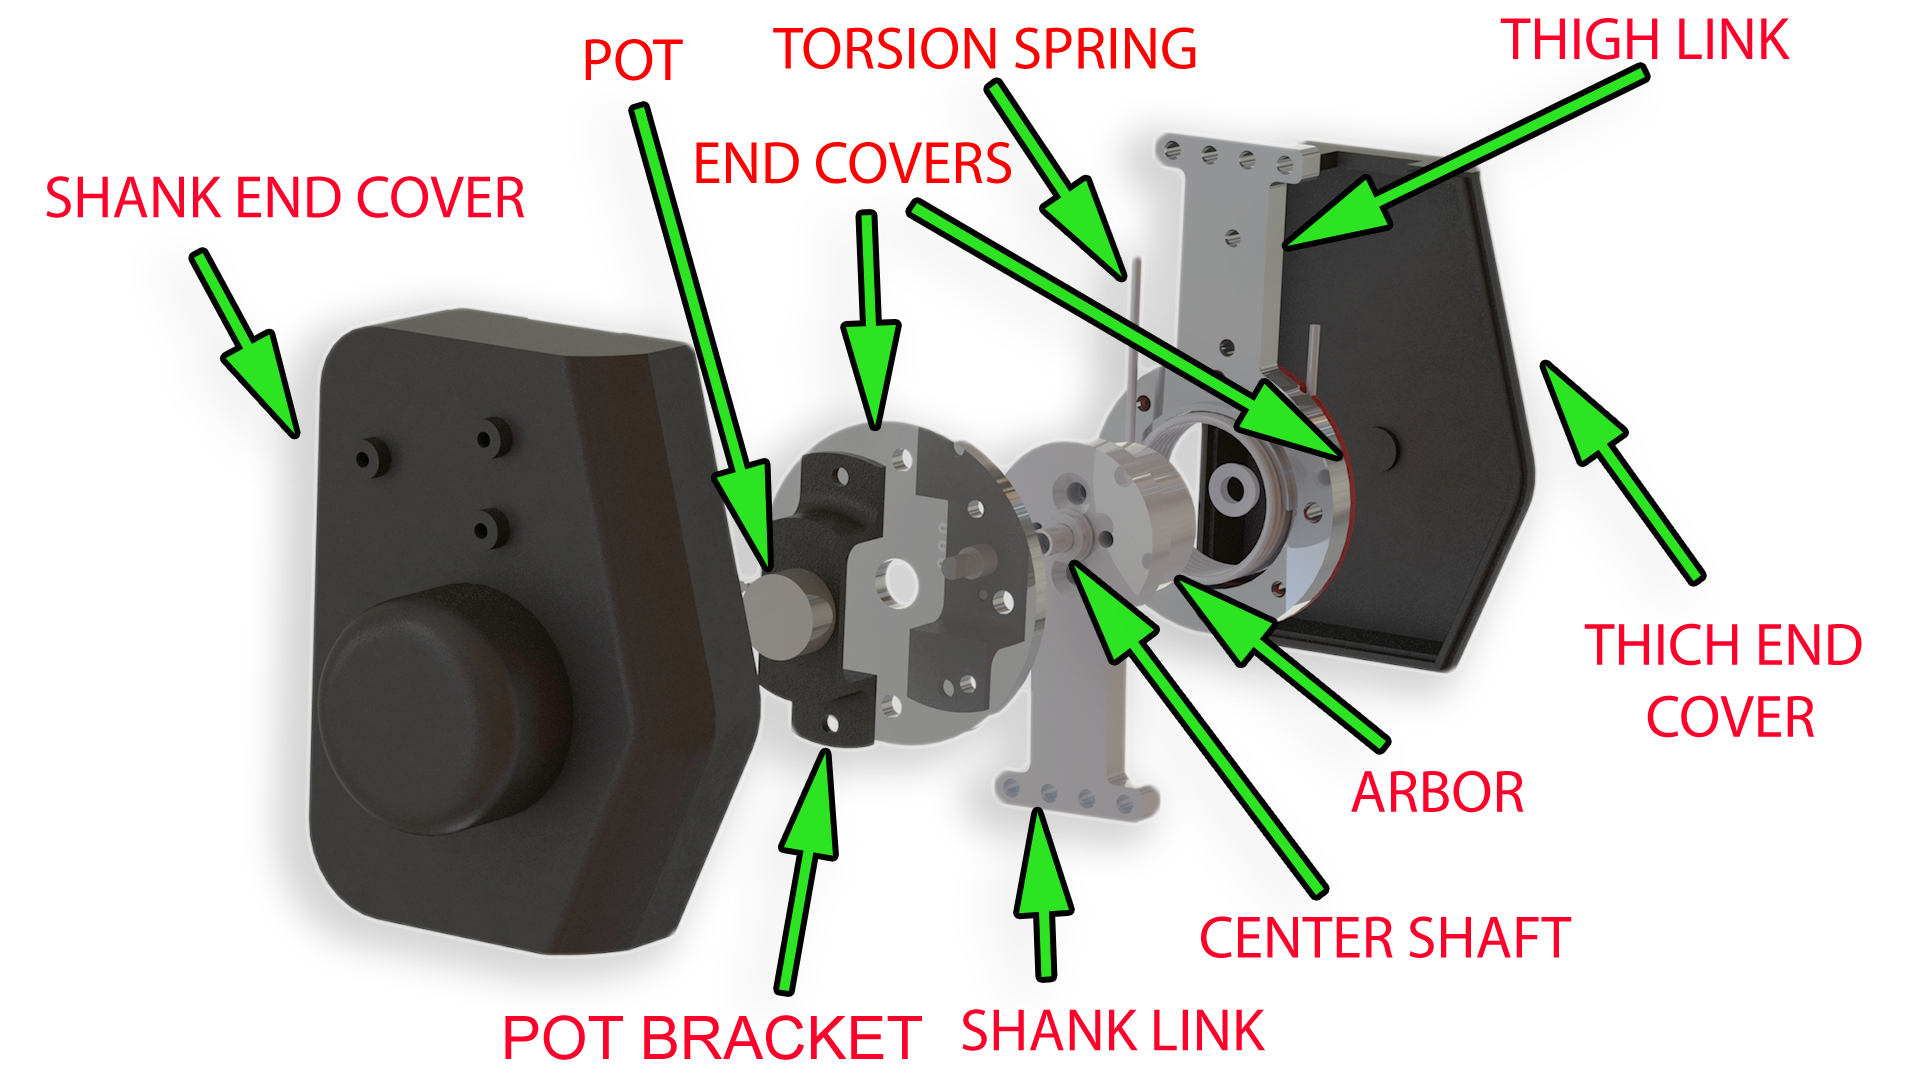
\includegraphics[scale=0.16]{images/mech_design/knee exploded view_edit2.png}}
        \caption[Custom Knee Mechanism]{The custom clutch/brake knee mechanism and the external housing. The covers keep the user safe from the potential sharp internal metal components. }
        \label{fig:kneemechASM}
    \end{subfigure}
    \begin{subfigure}{\textwidth}
        \centering
        \captionsetup{justification=centering}
        \centerline{
        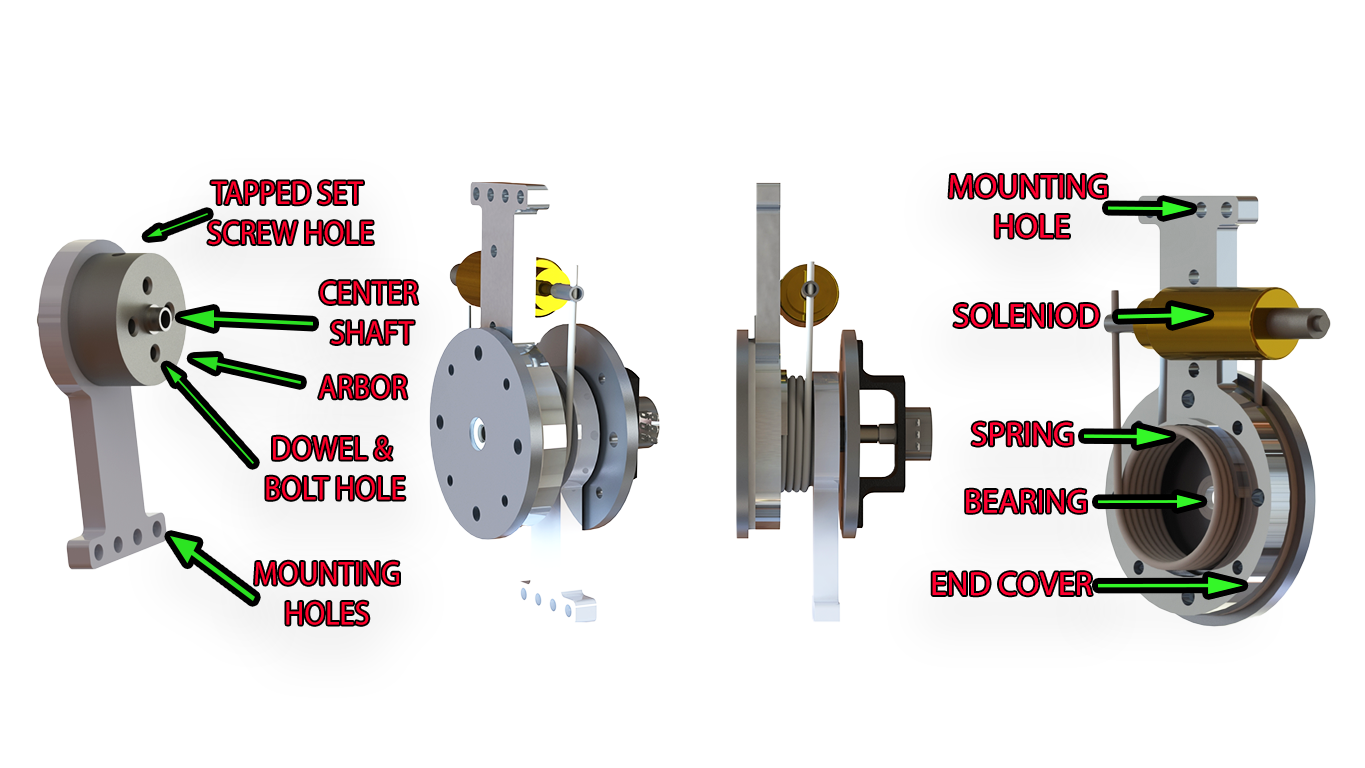
\includegraphics[scale=0.3]{images/mech_design/all_knee.png}}
        \caption[Wrap Spring Clutch Mechanism]{Wrap Spring Clutch Mechanism Sub Assemblies. The solenoid is used to push on the spring tang which enlargers the diameter of the spring  allowing free motion. The mounting hole connects the exoskeleton legs through the modular end cap. }
        \label{fig:subknee}
    \end{subfigure}    
    \caption{Exploded view of wrap spring clutch knee and the sub-assemblies.}
    \label{fig:kneemech}
\end{figure}

A similar approach represented in \cite{tung2013design} was followed to estimate the arbor diameter and the diametric interference for the design, which is the crucial part of the knee joint. The critical parameters of the knee were measured and summarized in \autoref{tab:KneeDesign}.

\begin{table}[h!]
\centering
 \begin{tabular}{|c || c|} 
 \hline
 Parameter & Value  \\ [0.5ex] 
 \hline\hline
 Spring Coil Inner Diameter   & $43.58132mm$ ($1.7158in$)   \\
\hline
Spring Wire Diameters &   $2.921mm$  ($0.115in$)  \\
\hline
Number of Turns     &   $6.5$ \\
\hline
Diametric Interference    &   $0.70358mm$ ($0.0277in$) \\
 \hline
  Arbor Diameter &  $44.2849mm$ ($1.7435 in$) \\ [1ex]
 \hline
 \end{tabular}
\caption[Knee Parameters]{Knee Design Parameters for the custom spring used in the final design.}
\label{tab:KneeDesign}
\end{table}


% \begin{tabular}{ |c||c| }
%  \hline
%  \multicolumn{2}{|c|}{Knee parameters} \\
%  \hline
% Spring Coil Inner Diameter   & $43.58132mm$ ($1.7158in$)   \\
% Spring Wire Diameters &   $2.921mm$  ($0.115in$)  \\
% Number of Turns     &   $6.5$ \\
% Diametric Interference    &   $0.70358mm$ ($0.0277in$) \\
%   Arbor Diameter (Spring Coil Inner Diameter + diametric interference) &  $44.2849mm$ ($1.7435 in$) \\
%  \hline
% \end{tabular}


% \noindent
% \begin{itemize}
% \item Spring Coil Inner Diameter: $43.58132mm$ ($1.7158in$)
% \item Spring Wire Diameter: $2.921mm$  ($0.115in$)
% \item Number of turns: $6.5$
% \item diametric interference: $0.70358mm$ ($0.0277in$)
% \item Arbor Diameter (Spring Coil Inner Diameter + diametric interference): $44.2849mm$ ($1.7435 in$)
% \end{itemize}


The arbor's initial design had a larger diameter than the spring's inner diameter to establish an interference between the spring and the arbor. This interference created an initial contact pressure, and when the arbor started to rotate, the frictional force started to increase. \autoref{eq:forces}  calculates the average and tangential forces across this region. The Normal and Tangential Forces are used to calculate the holding torque.

\begin{equation}
\large
\begin{aligned}
    \large
    F = pbrd\Phi + p_cbrd\Phi && \text{Normal Force}&\\
    p  = p_0 e^{\mu\Phi} && \text{ Result from Tangential Force}&
    \end{aligned}
\caption[Force Equations for Arbor]{Force Equations}
\label{eq:forces}
\end{equation}

where,
$p$ = total pressure 

$b$ = breadth of the wire 

$r$ = radius of the arbor 

$p_c$ = Centrifugal pressure 

$p_0$ = Initial pressure 

$\mu$ = Frictional coefficient

$d\Phi$ = small angle 

$\phi$ = total angle \\

During midstance, the relative motion between the shank and thigh links in the direction of knee flexion, causing the spring to wrap around the arbor, which produces the wrapping effect. The movement between the segments is locked during this condition, thus transferring the load to the ground. The brake has to be disengaged to allow free movement during the swing phase, and this is achieved using a linear actuator where the end of the actuator is connected to the spring's free leg. Thus by energizing the actuator, the spring can be unwound. This unwrapping effect of the spring disengages the brake and allows for free knee movement. This normally-closed brake ensures user safety during power failures, and its quasi-passive nature helps sustain the battery for longer cycles of gait. 

Several experiments were conducted in simulation and on the physical model to measure the knee's mechanical properties. The objective of the experiments was to document the properties and limitations of the wrap spring clutch knee. In \cite{SubraMani2020} the experiments are expanded in greater detail. 

A test-bed was designed to evaluate the braking torque characteristics and study the relationship between interference and contact forces. A potentiometer was used to measure the knee angle change and a load cell to evaluate the applied load. Based on the collected data, the holding torque of the knee was estimated.

The extension test-bed shown in \autoref{fig:Extent_test_bed} was designed to study the frictional force behavior in the knee extension direction. The force on the shank link increased by adding additional mass until the clutch slipped. The point that the system slipped is referred to as the deflection point.

\begin{figure}
\centering
 \includegraphics[scale=0.15]{images/mech_design/extension_set_up.png}
    \caption[Extension Test Bed]{Tested bed for extension testing for the wrap spring clutch knee. The moment arm was attached to then knee in extension to measure when the knee failed. The potentiometer co-axil with the knee record the knee angle and a load cell was used to measure the applied load. The sensors were read using an arduino  which was read by a computer over a serial port. }
    \label{fig:Extent_test_bed}
\end{figure}

This procedure was carried out for different interference values. The load values were substituted into \autoref{eq:ovTorque} to find the new interference values at which the slipped occurred.
\begin{equation}
    \large
    T_U & = p_0br^2(1 - e^{-N2\pi\mu})
\label{eq:ovTorque}
\end{equation}

The inner diameter of the spring is controlled by applying a force to the spring leg. Which also controls the interference between the arbor and spring. \autoref{fig:extension_test} shows the results of  
five different interference measurements. The black dots are the points of deflections for different spring openings. The $0push$ happens when the free spring leg is at its initial $0$ position. $1push$ happens when the spring leg is moved horizontally by a distance of $.313 in$ until $4push$.   

\begin{figure}[h!]
    \centering
    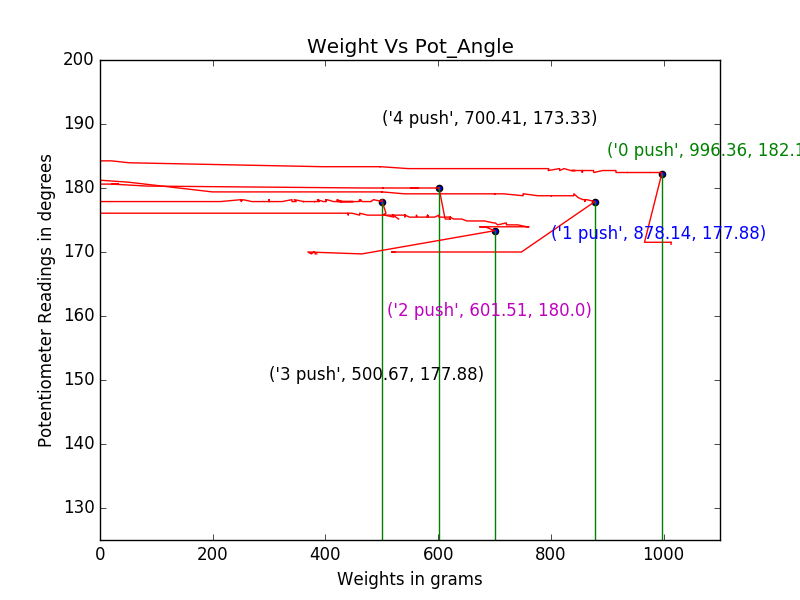
\includegraphics[scale=0.5]{images/mech_design/weighvspot.png}
    \caption[Knee Slipping Load Values]{Slipping Load values during Extension Test. The graphs shows the angle where the knee slipped vs the applied mass.}
    \label{fig:extension_test}
\end{figure} 


\autoref{fig:Flexion_test_bed} shows the flexion test-bed used to estimate the static and dynamic holding torque behavior of the knee joint. The load applied direction, and the knee flexion direction was along the direction of gravity. The load on the knee was applied at a distance of $0.46m$ from the knee center. The load was applied over several days to measure the durability of the system. This test-bed was utilized to find RoM and the brake release force.



\begin{figure}[h]
    \centering
    \includegraphics[scale=0.15]{images/mech_design/flexion_set_up.png}
    \caption[Flexion Test Bed]{Tested bed for flexion testing for the wrap spring clutch knee. The moment arm was attached to then knee in flexion and mass was added over time until the knee failed. The potentiometer co-axil with the knee record the knee angle over time over time The sensors were read using an arduino  which was read by a computer over a serial port.}
    \label{fig:Flexion_test_bed}
\end{figure}

The knee was loaded until the knee began to slip. The knee was found to have a maximum holding torque of $63Nm$, after which the knee started to slip. The knee was constructed to hold for an extended period of time, after which the knee lost 4$^{\circ}$ was observed, which was due to excessive stressing on the spring during maximum holding torque. The stress on the spring moved past its elastic region and entered the plastic region, due to which it was not able to coil back to its original position. \autoref{fig:loss_in_rom} shows the result of loss in the range of motion tests.
\begin{figure}[h!]
    \centering
    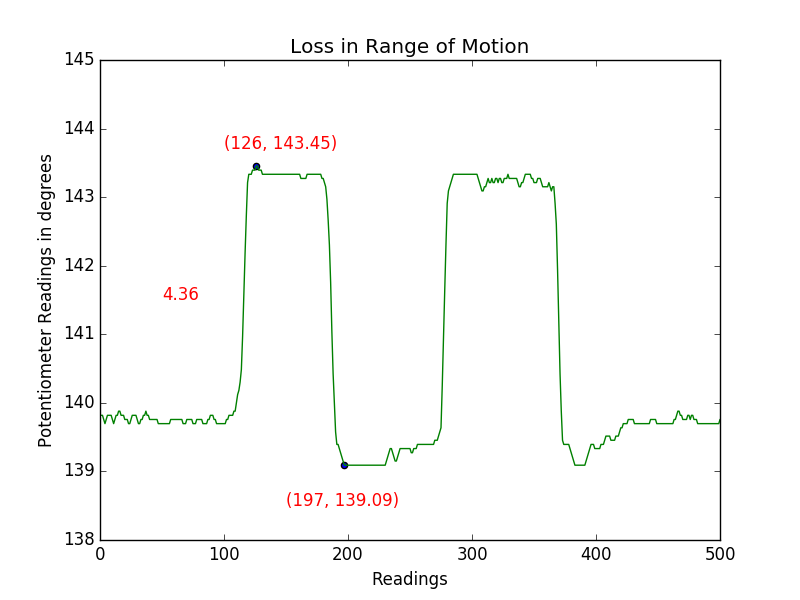
\includegraphics[scale=0.5]{ images/mech_design/loss_in_rom.png}
    \caption{Wrap Spring Clutch Knee Motion}{Loss in range of motion of the knee over time.}
    \label{fig:loss_in_rom}

\end{figure}

\autoref{fig:durabilitytest} shows the results of the durability test. During the test, the brake was engaged at three different loading conditions $48Nm$, $50Nm$, and $63Nm$. The brake was engaged to hold this position for four consecutive days, where the load between the days were increased; $48Nm$ on the first day, $50Nm$ for the second and third (since being the target requirement), and on the fourth day, we pushed the brake to the peak value of $63Nm$. The noise of the sensors was removed using a moving average filter.  The observed angular difference of the brake from the start of the test to the end was $0.75^{\circ}$.

\begin{figure}[h!]
    \centering
    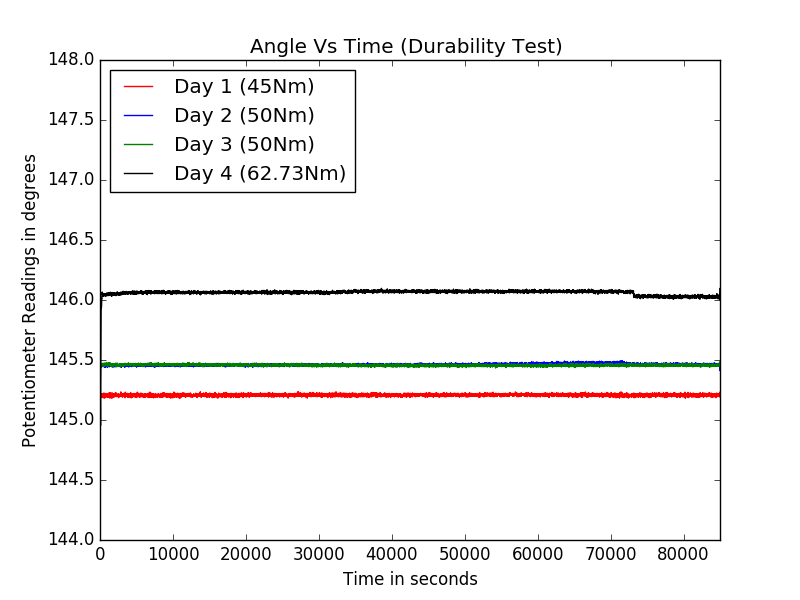
\includegraphics[scale=0.50]{images/mech_design/Durability_test.png}
    \caption{Durability Test of Wrap Spring Clutch Knee}{Change in angle of the wrap spring clutch knee over a four day period and increase in mass.}
    \label{fig:durabilitytest}
\end{figure}


The testing results demonstrated that it is possible to build an analytical-based design approach for an actuator using biomechanical and predefined specifications.


The wrap spring clutch knee used an analytical-based design approach for the actuator selection. The knee developed for the LARRE is inexpensive and weighs less than  $1kg$. The system can be easily serviced or repaired. The detailed analytical model was used to identify the relationship between the parameters manipulated to improve the system's overall performance. The wrap spring clutch/brake mechanism underwent a wide range of testing to measure all the necessary knee joint characteristics. 

% \begin{figure}
% \centering
%      \begin{subfigure}{.45\textwidth}
%         \centering
%           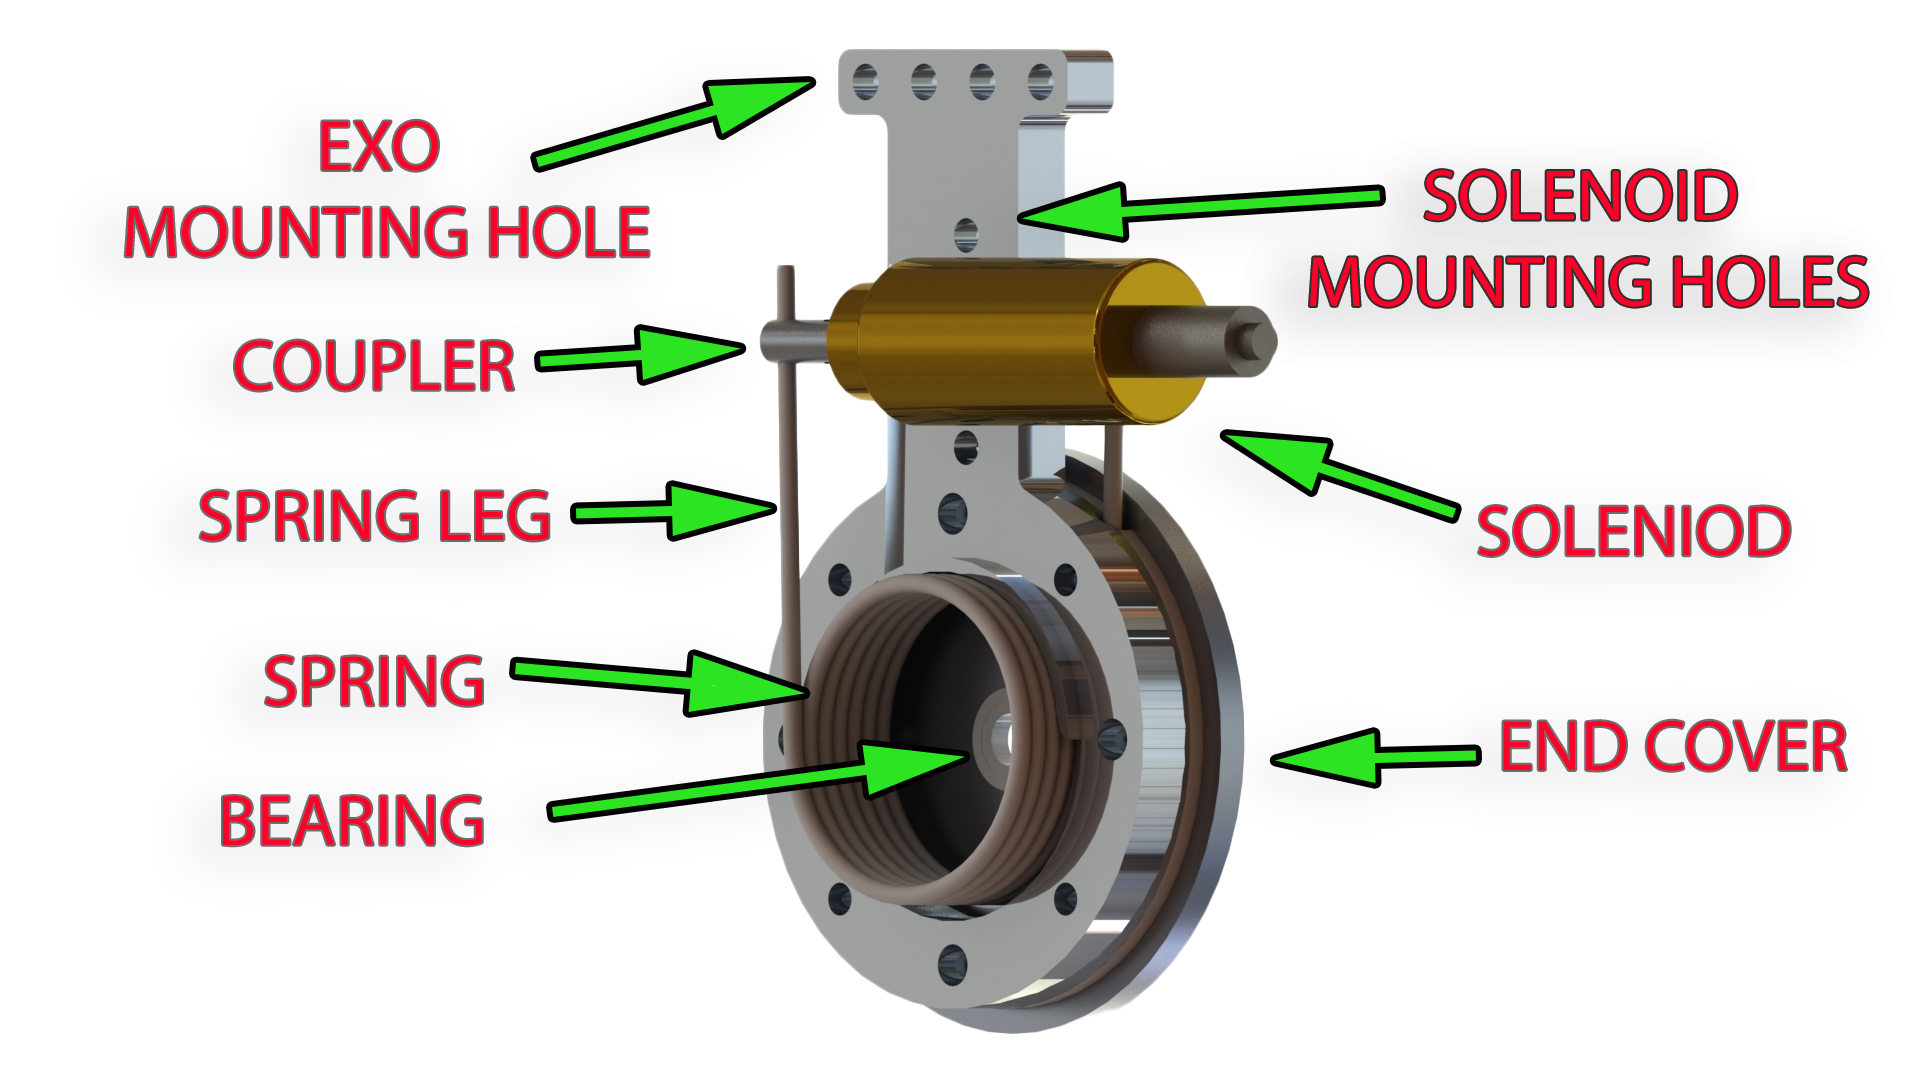
\includegraphics[ scale=0.10]{images/mech_design/thigh_assembly2.png}
%     \caption[Thigh Sub-Assembly]{Thigh Sub-assembly: all components are labeled. The solenoid controls the activation of the brake.}
%     \label{fig:thigh_sub}
%     \end{subfigure} 
%     %
%      \begin{subfigure}{.45\textwidth}
%         \centering
%         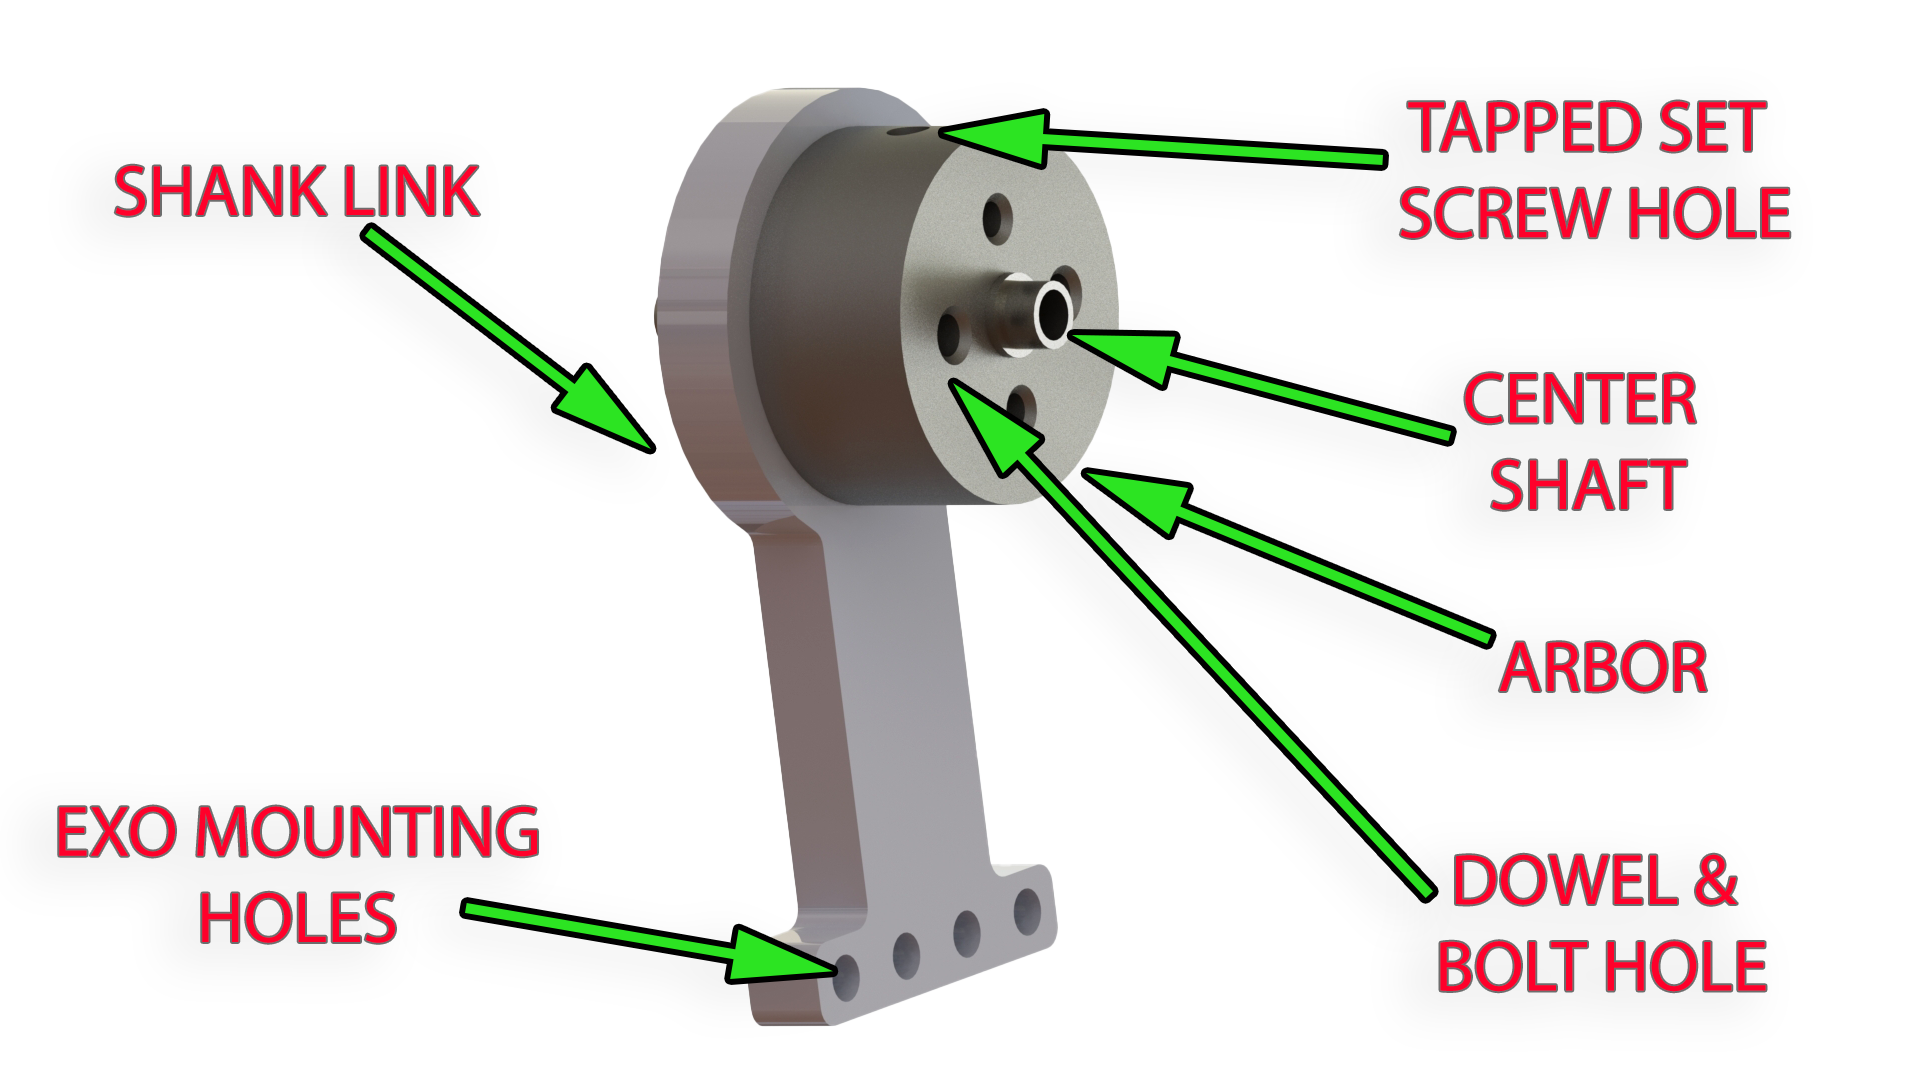
\includegraphics[ scale=0.10]{images/mech_design/shank_assembly2.png}
%         \caption[Shank Sub-Assembly]{Shank Sub-assembly: The arbor interfaces with the spring. When the spring closes, it grabs the arbor and prevents rotation.}
%         \label{fig:shank_sub}
%     \end{subfigure}
%     \caption[Knee Sub-Assemblies]{The Knee sub-assemblies}
%     \label{fig:sub_knee}
% \end{figure}
